\section[Section to try things] 	% Short Title for table of contens and headline
{Section to give examples for the application of this template} 	% Long title (only on start page of chapter)
\label{lasmREADME} 		% Label for cross refs
% ~~~~~~~~~~~~~~~~~~~~~~~~~~~~~~~~~~~~~~~~~~~~~~~~~
% ~~~~~~~~~~~~~~~~~~~~~~~~~~~~~~~~~~~~~~~~~~~~~~~~~
%
This is a chapter to try settings of template.
% ~~~~~~~~~~~~~~~~~~~~~~~~~~~~~~~~~~~~~~~~~~~~~~~~~  
\subsection{Test Text paragraphs \textbackslash par}
% ~~~~~~~~~~~~~~~~~~~~~~~~~~~~~~~~~~~~~~~~~~~~~~~~~
%
\blindtext
\par
\blindtext
%
% <<<<<<<<<<<<<<<< End of section  >>>>>>>>>>>>>>>> 	-> 5 empty comment lines (including this line)
%
%
%
%
% ~~~~~~~~~~~~~~~~~~~~~~~~~~~~~~~~~~~~~~~~~~~~~~~~~
\subsection{Bibliography: cite commands}
% ~~~~~~~~~~~~~~~~~~~~~~~~~~~~~~~~~~~~~~~~~~~~~~~~~
%
The source data for citation have to be in \textbf{Literature.bib}.
You can export these data for example from \textbf{citavi} using \emph{Datei/Exportieren}.
Further information on LaSM Wiki.
\\
\textbackslash cite\{Cremer.1967\}: \cite{Cremer.1967}\\
\textbackslash textcite\{Cremer.1967\}: \textcite{Cremer.1967}\\
\textbackslash citeauthor\{Cremer.1967\}: \citeauthor{Cremer.1967}\\
\textbackslash parencite\{Cremer.1967\}: \parencite{Cremer.1967}\\
\textbackslash parencite*\{Cremer.1967\}: \parencite*{Cremer.1967}\\
\par
Examples for additional options for page numbers etc.\\
\textbackslash textcite[\textbackslash pno~59]\{Cremer.1967\}: \textcite[\pno~59]{Cremer.1967}\\
\textbackslash parencite[see][59--63]\{Cremer.1967\}: \parencite[see][59--63]{Cremer.1967}\\
\par
The number of author names used in the text with these cite commands can be adjusted in the \textbf{GlobalStyle.sty}:\\
Just change the number of \textbf{maxcitenames} in the \textbf{\textbackslash ExecuteBibliographyOptions}\\
\par
To change the brackets from round ( ) to square [ ], there are four code lines in the BIBLATEX section in the \textbf{GlobalStyle.sty}.
\par
\parencite{ISO162831:2014}
%
% <<<<<<<<<<<<<<<< End of section  >>>>>>>>>>>>>>>> 	-> 5 empty comment lines (including this line)
%
%
%
%
% ~~~~~~~~~~~~~~~~~~~~~~~~~~~~~~~~~~~~~~~~~~~~~~~~~
\subsection{Acronyms}
\label{Acro}
% ~~~~~~~~~~~~~~~~~~~~~~~~~~~~~~~~~~~~~~~~~~~~~~~~~
%
\noindent
Command: \textbackslash acf\{...\}: \acf{FRF}\\
Command: \textbackslash acs\{...\}: \acs{FRF}\\
Command: \textbackslash ac\{...\} first time: \ac{B}\\
Command: \textbackslash ac\{...\} second time: \ac{B}\\
For plural  use command: \textbackslash acp\{...\}: \acp{FRF}
%
% <<<<<<<<<<<<<<<< End of section  >>>>>>>>>>>>>>>> 	-> 5 empty comment lines (including this line)
%
% ~~~~~~~~~~~~~~~~~~~~~~~~~~~~~~~~~~~~~~~~~~~~~~~~~
\subsection{Tables}
% ~~~~~~~~~~~~~~~~~~~~~~~~~~~~~~~~~~~~~~~~~~~~~~~~~
To create tables without a *.csv file, \url{http://www.tablesgenerator.com/} is recommended.
For professional tables \textbf{bootabs table style} is also recommended.
Example see \ref{SampleTable}
%
\begin{table}[htb]
	\centering
	\caption{Normale Tabelle mit dem booktabs Stil}
	\label{SampleTable}
	\begin{tabular}{@{}lllll@{}}
		\toprule
		& A & B  & C  & D  \\ \midrule
		a & 1 & 2  & 3  & 4  \\
		b & 5 & 6  & 7  & 8  \\
		c & 9 & 10 & 11 & 12 \\ \bottomrule
	\end{tabular}
\end{table}
%
% %
% \subsubsection{Table with footnotes using the threepartable package}
% % 
 To add footnotes to tables use the threeparttable environment.
 %
 \begin{table}[htb]
 	\centering
 	\begin{threeparttable}
 		%
 		\caption[Table with footnotes]{Table with footnotes}
 		\label{tab:anytab}
 		%
 		\begin{tabular}{@{}llr@{}} \toprule
 			\multicolumn{2}{c}{Item} \\ \cmidrule(r){1-2}
 			Animal 		& Description 	& Price (\$)\\ \midrule
 			Gnu\tnote{a}& stuffed   	& 92.50 \\
 			Emu\tnote{b}& stuffed   	& 33.33 \\\bottomrule
 		\end{tabular}
 		%
 		\begin{tablenotes}
 			\item[a]	\footnotesize	any bla
 			\item[b]	\footnotesize	any blabla
 		\end{tablenotes}
 		%
 	\end{threeparttable}
 \end{table}
% %
% % <<<<<<<<<<<<<<<< End of section  >>>>>>>>>>>>>>>> 	-> 5 empty comment lines (including this line)
% %
% %
% %
% %% ~~~~~~~~~~~~~~~~~~~~~~~~~~~~~~~~~~~~~~~~~~~~~~~~~
\subsection{Units and numbers}
% ~~~~~~~~~~~~~~~~~~~~~~~~~~~~~~~~~~~~~~~~~~~~~~~~~
%
Units and numbers in the text and equations can be set using the following commands (see \url{https://www.ctan.org/pkg/siunitx}):
\\
\textbackslash si  \{\textbackslash metre \textbackslash per \textbackslash square \textbackslash second \} gives \si{\metre \per \square \second}
\\
\textbackslash SI  \{1e-2\} \{\textbackslash metre \textbackslash per \textbackslash newton \textbackslash per \textbackslash second\} gives \SI{1e-2}{\metre\per\newton\per\second}
\\
\textbackslash SIrange  \{1e-4\} \{1e-2\} \{\textbackslash metre \textbackslash per \textbackslash newton \textbackslash per \textbackslash second\} gives \SIrange{1e-4}{1e-2}{\metre\per\newton\per\second}
\\
\textbackslash num  \{1e-2\} gives \num{1e-2}


% %% ~~~~~~~~~~~~~~~~~~~~~~~~~~~~~~~~~~~~~~~~~~~~~~~~~
\subsection{Symbols}
% ~~~~~~~~~~~~~~~~~~~~~~~~~~~~~~~~~~~~~~~~~~~~~~~~~
%
The usage is similar to the Acronyms (section \ref{Acro})\\
Command: \textbackslash acs\{LW\} gives \acs{LW}
\\
Command: \textbackslash acs\{V\} \textbackslash acs\{subRR\} gives \acs{V}\acs{subRR}
\\
Symbols are predefined in the list of Symbols:\\
13-Frontmatter/Symbols.tex
\\
Own new symbols can be added to this list. 
Only Symbols that are used in the document appear in the list of symbols.


% ~~~~~~~~~~~~~~~~~~~~~~~~~~~~~~~~~~~~~~~~~~~~~~~~~
\subsection{Equations}
% ~~~~~~~~~~~~~~~~~~~~~~~~~~~~~~~~~~~~~~~~~~~~~~~~~
%
Hello, here is some text without a meaning. This text should show what
a printed text will look like at this place. If you read this text, you will
get no information. Really?
%
\begin{equation}
\acs{LW}_{,k}=10\lg\left( \frac{\sum_{j=1}^J W_{\mathrm{NB},k,j}}{W_{0}}\right) 
\label{L_W,k}
\end{equation}
%
Without using \textbackslash par. Is there no information? Is there a difference
between this text and some nonsense like “Huardest gefburn”? Kjift –
not at all! A blind text like this gives you information about the selected
font, how the letters are written and an impression of the look. This text
should contain all letters of the alphabet and it should be written in of the
original language. There is no need for special content, but the length of
words should match the language.
\par
Hello, here is some text without a meaning. This text should show what
a printed text will look like at this place. If you read this text, you will
get no information. Really?
%
\begin{equation}
\acs{LW}_{,k}=10\lg\left( \frac{\sum_{j=1}^J W_{\mathrm{NB},k,j}}{W_{0}}\right) 
\label{L_Wa,k}
\end{equation}
%
\par
With \textbackslash par after equation. Is there no information? Is there a difference
between this text and some nonsense like “Huardest gefburn”? Kjift –
not at all! A blind text like this gives you information about the selected
font, how the letters are written and an impression of the look. This text
should contain all letters of the alphabet and it should be written in of the
original language. There is no need for special content, but the length of
words should match the language.
%
% <<<<<<<<<<<<<<<< End of section  >>>>>>>>>>>>>>>> 	-> 6 empty comment lines (including this line)
%
%
 % ~~~~~~~~~~~~~~~~~~~~~~~~~~~~~~~~~~~~~~~~~~~~~~~~~
 \subsection{Lists} 			% Long title
 % ~~~~~~~~~~~~~~~~~~~~~~~~~~~~~~~~~~~~~~~~~~~~~~~~~
 %
 List are basic elements in a document, when used correctly they keep concepts organized and structured. This section explains how to create and modify numbered and unnumbered lists in \LaTeX. 
 %
 % <<<<<<<<<<<<<<<< End of section  >>>>>>>>>>>>>>>> 	-> 6 empty comment lines (including this line)
 %
 %
 %
 %
 % ~ ~ ~ ~ ~ ~ ~ ~ ~ ~ ~ ~ ~ ~ ~ ~ ~ ~ ~ ~ ~ ~ ~ ~ ~ 
 \subsubsection{Ordered lists} 		% Long title
 % ~ ~ ~ ~ ~ ~ ~ ~ ~ ~ ~ ~ ~ ~ ~ ~ ~ ~ ~ ~ ~ ~ ~ ~ ~ 
 %
 \begin{enumerate}
 	\item The labels consists of sequential numbers.
 	\item The numbers starts at 1 with every call to the enumerate environment.
 \end{enumerate}
 %
 % <<<<<<<<<<<<<<< End of subsection >>>>>>>>>>>>>>>  	-> 5 empty comment lines (including this line)
 %
 %
 %
 % ~ ~ ~ ~ ~ ~ ~ ~ ~ ~ ~ ~ ~ ~ ~ ~ ~ ~ ~ ~ ~ ~ ~ ~ ~ 
 \subsubsection{Unordered lists} 		% Long title
 % ~ ~ ~ ~ ~ ~ ~ ~ ~ ~ ~ ~ ~ ~ ~ ~ ~ ~ ~ ~ ~ ~ ~ ~ ~ 
 %
 \begin{itemize}
 	\item The individual entries are indicated with a black dot, a so-called bullet.
 	\item The text in the entries may be of any length.
 \end{itemize}
 %
 % <<<<<<<<<<<<<<< End of subsection >>>>>>>>>>>>>>>  	-> 5 empty comment lines (including this line)
 %
 %
 %
 % ~ ~ ~ ~ ~ ~ ~ ~ ~ ~ ~ ~ ~ ~ ~ ~ ~ ~ ~ ~ ~ ~ ~ ~ ~ 
 \subsubsection{Nested lists} 		% Long title
 % ~ ~ ~ ~ ~ ~ ~ ~ ~ ~ ~ ~ ~ ~ ~ ~ ~ ~ ~ ~ ~ ~ ~ ~ ~ 
 %
 \begin{enumerate}
 	\item The labels consists of sequential numbers.
 	\begin{itemize}
 		\item The individual entries are indicated with a black dot, a so-called bullet.
 		\item The text in the entries may be of any length.
 	\end{itemize}
 	\item The numbers starts at 1 with every call to the enumerate environment.
 \end{enumerate}
 %
 % <<<<<<<<<<<<<<< End of subsection >>>>>>>>>>>>>>>  	-> 5 empty comment lines (including this line)
 %
 %
 %
 % ~ ~ ~ ~ ~ ~ ~ ~ ~ ~ ~ ~ ~ ~ ~ ~ ~ ~ ~ ~ ~ ~ ~ ~ ~ 
 \subsubsection{List styles: ordered lists} 		% Long title
 % ~ ~ ~ ~ ~ ~ ~ ~ ~ ~ ~ ~ ~ ~ ~ ~ ~ ~ ~ ~ ~ ~ ~ ~ ~ 
 %
 The default numbering scheme is: 
 \begin{itemize}
 	\item Arabic number (1, 2, 3, ...) for Level 1 
 	\item Lowercase letter (a, b, c, ...) for Level 2 
 	\item Lowercase Roman numeral (i, ii, iii, ...) for Level 3 
 	\item Uppercase letter (A, B, C, ...) for Level 4. 
 \end{itemize}
 These numbers can be changed by redefining the commands that typeset the numbers of various list levels. For example: 
 \renewcommand{\labelenumii}{\Roman{enumii}}
 \begin{enumerate}
 	\item First level item
 	\item First level item
 	\begin{enumerate}
 		\item Second level item
 		\item Second level item
 		\begin{enumerate}
 			\item Third level item
 			\item Third level item
 			\begin{enumerate}
 				\item Fourth level item
 				\item Fourth level item
 			\end{enumerate}
 		\end{enumerate}
 	\end{enumerate}
 \end{enumerate}
 The command must be placed in the preamble to change the labels globally or right before \textbackslash begin\{enumerate\} to change labels only in this list.
 %
 % <<<<<<<<<<<<<<< End of subsection >>>>>>>>>>>>>>>  	-> 5 empty comment lines (including this line)
 %
 %
 %
 % ~ ~ ~ ~ ~ ~ ~ ~ ~ ~ ~ ~ ~ ~ ~ ~ ~ ~ ~ ~ ~ ~ ~ ~ ~ 
 \subsubsection{List styles: unordered lists} 		% Long title
 % ~ ~ ~ ~ ~ ~ ~ ~ ~ ~ ~ ~ ~ ~ ~ ~ ~ ~ ~ ~ ~ ~ ~ ~ ~ 
 %
 The default numbering scheme is: 
 \begin{itemize}
 	\item Level 1 is \textbullet, 
 	\item Level 2 is \textendash, 
 	\item Level 3 is \textasteriskcentered 
 	\item Level 4 is \textperiodcentered. 
 \end{itemize}
 These labels can be changed by redefining the commands that typeset them for various list levels. For example, to change Level 1 to black square and Level 2 to white square we'll use : 
 \renewcommand{\labelitemi}{o}
 \renewcommand\labelitemii{x}
 \begin{itemize}
 	\item  First Level
 	\begin{itemize}
 		\item  Second Level
 		\begin{itemize}
 			\item  Third Level
 			\begin{itemize}
 				\item  Fourth Level
 			\end{itemize}
 		\end{itemize}
 	\end{itemize}
 \end{itemize}
 You can also change the item label for a specific entry, for example: 
 \begin{itemize}
 	\item  Default item label for entry one
 	\item  Default item label for entry two
 	\item[x]  Custom item label for entry three
 \end{itemize}
 The command must be placed in the preamble to change the labels globally or right before \textbackslash begin\{itemize\} to change labels only in this list.
 %
 % <<<<<<<<<<<<<<<< End of section  >>>>>>>>>>>>>>>> 	-> 6 empty comment lines (including this line)
 %
 %
 %
 %
 % ~~~~~~~~~~~~~~~~~~~~~~~~~~~~~~~~~~~~~~~~~~~~~~~~~
 \subsection{Using commands from Commands.sty} 			% Long title
 % ~~~~~~~~~~~~~~~~~~~~~~~~~~~~~~~~~~~~~~~~~~~~~~~~~
 %
 \noindent
 Set up commands in the Commands.sty file:\\
 Example:\\
 Code in Commands.sty:\\
 \textbackslash newcommand\{\textbackslash matlab\}\{\textbackslash textsc\{Matlab\}\textbackslash xspace\}\\
 Use the following the text:\\
 I was using \textbackslash matlab througout.: I was using \matlab througout.
 %
 % <<<<<<<<<<<<<<<< End of section  >>>>>>>>>>>>>>>> 	-> 6 empty comment lines (including this line)
 %
 
 % ~~~~~~~~~~~~~~~~~~~~~~~~~~~~~~~~~~~~~~~~~~~~~~~~~
 \subsection{ToDoNotes}
 % ~~~~~~~~~~~~~~~~~~~~~~~~~~~~~~~~~~~~~~~~~~~~~~~~~
 %
 Useful to highlight todos during the writing process.
 Using the command \\
 \textbackslash listoftodos
 \\
 creates a list of all todos in the document.
 \\
 \todo[inline]{This is a to do note in line}
 \todo[]{this is a to do note on the margin of the page}
 %
 % <<<<<<<<<<<<<<<< End of section  >>>>>>>>>>>>>>>> 	-> 5 empty comment lines (including this line)
 %
 %
 %
 %
 %
 % ~~~~~~~~~~~~~~~~~~~~~~~~~~~~~~~~~~~~~~~~~~~~~~~~~  
 \subsection{Add multiple figures using minipage}
 % ~~~~~~~~~~~~~~~~~~~~~~~~~~~~~~~~~~~~~~~~~~~~~~~~~
 %
 This example shows three figures that are arranged in two columns.
 One figure in the left column and two on top of each other in the right column, such that they are aligned with the upper and lower boundary of the figure in the left column.
 To align the figures the hight of the minipage must be the same for the left and right minipage.
 The height of the left minipage must be adjusted with respect to the aspect ratio of the figure.
 To align the figures in the right minipage vfil is used to use all the available vertical space between the two.
 The sum of the minipage with should be smaller than the full textwidth.
 %
 \begin{figure}[htb]
 	\centering
 	%
 	% \begin{minipage}[outer position][{]height][inner position]{width}
 	%
 	% LEFT MINIPAGE WITH ONE FIGURE
 	\begin{minipage}[c][0.525\columnwidth][c]{0.70\columnwidth} 	% 0.60 x 3/4 = 0.45
 		% Height and width should be adjusted to the figure aspect ratio
 		% In this case the figure is 3/4, hence 
 		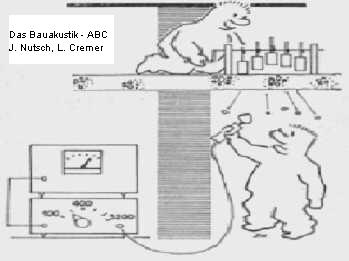
\includegraphics[width=\linewidth]{\GraficPath SampleFigs/Schall_Messtechnik}
 	\end{minipage}
 	%
 	\hfil%
 	% RIGHT MINIPAGE WITH TWO FIGURES
 	\begin{minipage}[c][0.525\columnwidth][c]{0.25\columnwidth}  % same height as left minipage chosen --> 0.525
 		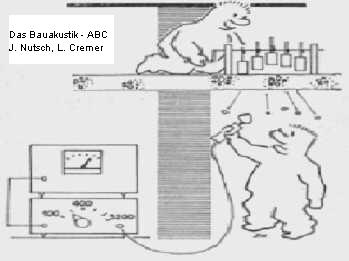
\includegraphics[width=\linewidth]{\GraficPath SampleFigs/Schall_Messtechnik}%
 		\\
 		\vfill
 		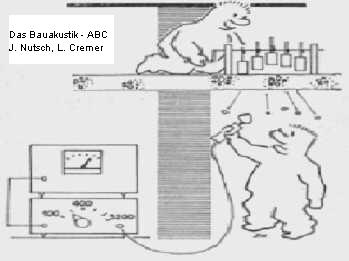
\includegraphics[width=\linewidth]{\GraficPath SampleFigs/Schall_Messtechnik}
 	\end{minipage}
 	%
 	\caption[Kurztitel]{Multiple figures using minipage}
 	\label{fig:ArtificialSourceOneFoot}
 \end{figure}
 %
 % <<<<<<<<<<<<<<<< End of section  >>>>>>>>>>>>>>>> 	-> 6 empty comment lines (including this line)
 %
 %
 %
 %
 % ~~~~~~~~~~~~~~~~~~~~~~~~~~~~~~~~~~~~~~~~~~~~~~~~~  
 \subsection{Add figures with the subcaption package}
 % ~~~~~~~~~~~~~~~~~~~~~~~~~~~~~~~~~~~~~~~~~~~~~~~~~
 %
 \begin{figure}[htb]
 	\centering
 	\subcaptionbox{Figure A\label{LabelOfFigureA}}
 	{\includegraphics[width=0.4\linewidth]{\GraficPath Logo-THRo} }
 	\subcaptionbox{Figure B\label{LabelOfFigureB}}
 	{
\includegraphics[width=0.4\linewidth]{\GraficPath SampleFigs/Logo-NawaRo} }
 	\caption[subcaption]{subcaption}\label{FigureAB}
 \end{figure}
 %
 % <<<<<<<<<<<<<<<< End of section  >>>>>>>>>>>>>>>> 	-> 5 empty comment lines (including this line)
 %
 %
 %
 %
 % ~~~~~~~~~~~~~~~~~~~~~~~~~~~~~~~~~~~~~~~~~~~~~~~~~  
 \subsection{Include svg}
 % ~~~~~~~~~~~~~~~~~~~~~~~~~~~~~~~~~~~~~~~~~~~~~~~~~
% %
% \begin{figure}[htb]
% 	\centering
% 	\setlength\fwidth{0.7\columnwidth}
% 	\includesvg[width=\fwidth]{\GraficPath SampleFigs/Example-svg}
% 	\caption{SVG in sub directory}
% \end{figure}
% %
% \begin{figure}[htb]
% 	\centering
% 	\setlength\fwidth{0.7\columnwidth}
% 	\includesvg[angle=15,width=\fwidth]{\GraficPath SampleFigs/Example-svg}
% 	\caption{rotated SVG in sub directory}
% \end{figure}

\todo[inline]{Include svg funktioniert noch nicht}

 %
 % <<<<<<<<<<<<<<<< End of section  >>>>>>>>>>>>>>>> 	-> 5 empty comment lines (including this line)
 %
 %
 %
 %
 % ~~~~~~~~~~~~~~~~~~~~~~~~~~~~~~~~~~~~~~~~~~~~~~~~~  
 \subsection{Draw over image}
 % ~~~~~~~~~~~~~~~~~~~~~~~~~~~~~~~~~~~~~~~~~~~~~~~~~
 %
 Examples:\\
 Figure \ref{DrawOverImage}
% Figure \ref{DrawOverImageUsingCallouts}
 %
 \begin{figure}[htb]
 	\centering
 	\begin{tikzpicture}
 		\setlength\fwidth{0.7\columnwidth}
 		\node[anchor=south west,inner sep=0] (Bild) at (0,0)
 		{\includegraphics[width=\fwidth]{\GraficPath Logo-THRo}};
 		\begin{scope}[x=(Bild.south east),y=(Bild.north west)]
 			\draw[mycolor1, \LWd, \LSb] (0,0) rectangle (1,1);
 			\draw[] (0.5,0.6) node[anchor=north]{$text over image im math mode$};
 		\end{scope}
 	\end{tikzpicture}
 	\caption{draw over image using the scope environment}
 	\label{DrawOverImage}
 \end{figure}
 %
% \begin{figure}[htb]
% 	\centering
% 	\begin{annotate}
% 		{\includegraphics[width=0.4\columnwidth]{\GraficPath Logo-THRo}}{0.4}
% 		%\helpgrid
% 		\callout{2,2}{Callout}{0,0}
% 	\end{annotate}
% \caption{draw over image using the callouts package}
% \label{DrawOverImageUsingCallouts}
% \end{figure}
 %
 % <<<<<<<<<<<<<<<< End of section  >>>>>>>>>>>>>>>> 	-> 5 empty comment lines (including this line)
 %
 %
 %
 %

 
 % ~~~~~~~~~~~~~~~~~~~~~~~~~~~~~~~~~~~~~~~~~~~~~~~~~  
 \subsection{Sketches using tikz}
 % ~~~~~~~~~~~~~~~~~~~~~~~~~~~~~~~~~~~~~~~~~~~~~~~~~
 %
 \subsubsection{Example to use loops in tikz}
 % ~ ~ ~ ~ ~ ~ ~ ~ ~ ~ ~ ~ ~ ~ ~ ~ ~ ~ ~ ~ ~ ~ ~ ~ ~
 %
 \begin{figure}
 \centering
     % \input{./Figures/Tikz_test.tex}
     % \fbox{                                    % OPEN BOX AROUND TIKZ
     \begin{tikzpicture}
     \setlength\fwidth{0.7\columnwidth}
   	%
     % Varibles for sketch
     \newcommand{\FrameOutside}{100}
     \newcommand{\WallWidth}{506}
     \newcommand{\WallHeight}{259}
     \newcommand{\StudSpac}{62.5}
     \newcommand{\StudWidth}{6}
     \newcommand{\DimOffset}{50}
     \newcommand{\DimOffsetB}{10}
     %
     %
     \begin{axis}[%
     hide axis,
     width=\fwidth,   
     height=(\WallHeight+2*\FrameOutside)/(\WallWidth+2*\FrameOutside)*\fwidth,
     scale only axis,
     xmin=-\FrameOutside,
     xmax=\WallWidth+\FrameOutside,
     ymin=-\FrameOutside,
     ymax=\WallHeight+\FrameOutside,
     xmajorgrids=false,
     ]
  	%
     % Bars at top and bottom    
     \draw[gray, thin] 
     (0,0) rectangle (\WallWidth,\StudWidth);
     \draw[gray, thin] 
     (0,\WallHeight-\StudWidth) rectangle (\WallWidth,\WallHeight);
     % Studs
     \draw[gray, thin] \foreach \i in {0,1,2,...,8} 
     {(\i*\StudSpac,\StudWidth) rectangle 
     (\i*\StudSpac+\StudWidth,\WallHeight-\StudWidth)};
 	%
     % Dimensions
     \draw[latex-latex] 
     (0,\WallHeight+\DimOffset) -- (\WallWidth,\WallHeight+\DimOffset) node[midway,above]{\small \WallWidth \,cm};    
     \draw[black, thin] 
     (0,\WallHeight+\DimOffsetB) -- (0,\WallHeight+\DimOffset+\DimOffsetB);
     \draw[black, thin] 
     (\WallWidth,\WallHeight+\DimOffsetB) -- (\WallWidth,\WallHeight+\DimOffset+\DimOffsetB);
     %
     \draw[latex-latex] 
     (-\DimOffset,0) -- (-\DimOffset,\WallHeight) node[midway,above,rotate=90]{\small \WallHeight \,cm};
     \draw[black, thin] 
     (-\DimOffset-\DimOffsetB,0) -- (-\DimOffsetB,0);
     \draw[black, thin] 
     (-\DimOffset-\DimOffsetB,\WallHeight) -- (-\DimOffsetB,\WallHeight);
 	%
     \end{axis}
 	%
 	%
     \end{tikzpicture}
     % }                                         % CLOSE BOX AROUND TIKZ
 %
 \caption[Short figure caption]{Long figure caption}
 \label{fig:Tikz_test}
 \end{figure}
 %
 %
 \subsubsection{Example for plots in tikz}
 % ~ ~ ~ ~ ~ ~ ~ ~ ~ ~ ~ ~ ~ ~ ~ ~ ~ ~ ~ ~ ~ ~ ~ ~ ~
 If numeric data are available, it has some advantages to use \emph{tikz} graphics. An example is given in the file. 
 This file should not have thousands of data points.
 The global properties of the apperances of fonts, axis can be used from \textbf{PlotProperties}.
 \begin{figure}[htb]
 	\raggedright
 	\hspace{\LeftHspace}
 	%\setlength\fwidth{0.6\linewidth}    % Relative Breite des Diagramms  
 	%\centering                          % Zentrieren des Bildes
 	% This file was created by matlab2tikz.
%
% ADDITIONAL INFORMATION FOR THIS DATASET:
% --------------------------------------
% PATH: N:\01_FuE\07_NawaRo\SEA\TransmissionLossCB16\
% FILENAME: ExpVsSEAModellFPY2-EMODadj-TL-plot.fig
% LAST MODIFIED: 16-Jan-2018 19:33:38
% FIGURE NAME: n:\01_FuE\07_NawaRo\SEA\TransmissionLossCB16\ExpVsSEAModellFPY2-EMODadj.txt-TL-plot
% ANNOTATIONS: VAOne Datei 16mmSpanplatte_Nusser.va1
%               
%               
%               
%               
% --------------------------------------
%
%\definecolor{mycolor1}{rgb}{0.00000,0.44700,0.74100}%
%\definecolor{mycolor2}{rgb}{0.85000,0.32500,0.09800}%
%
\begin{tikzpicture}[trim axis left]
\begin{semilogxaxis}[%
soundreductionR axis style, % Default parameter for axis, look at: 13-Frontmatter/PlotProperties.sty
]
\addplot [color=mycolor1,LMa]
table[row sep=crcr]{%
	50	20.1\\
	63	16.6\\
	80	14\\
	100	20.4\\
	125	18.7\\
	160	20.8\\
	200	23.2\\
	250	25.3\\
	315	25.8\\
	400	26.8\\
	500	27.6\\
	630	28.4\\
	800	30\\
	1000	31.3\\
	1250	32.2\\
	1600	31.8\\
	2000	27\\
	2500	23.4\\
	3150	26.7\\
	4000	29.1\\
	5000	32.2\\
};
\addlegendentry{Messung FPY2};


\end{semilogxaxis}
\end{tikzpicture}%
 	\caption[Kurztitel]{Vergleich der Schalldämmung aus SEA-Modell und Messung. Einschalige Wand \SI{1.98 x 0.95}{\m} aus einer \SI{16}{\milli\m} Spanplatte ($\acs{rho}=\SI{646}{\kg\per\m\cubed}$; $\acs{E}\,=\,\SI{1890}{\mega\pascal}$;  $\acs{mu}=\num{0.3} $; $\acs{eta}\acs{subint}=\num{0.01}$). Das Volumen des Senderaumes beträgt $\acs{V}\acs{subSR}=\SI{54}{\m\cubed}$ und des Empfangsraumes $\acs{V}\acs{subRR}=\SI{70}{\m\cubed}$.  Die Messergebnisse stammen aus \parencite[222]{Nusser.2007}. Dort wird für den Prüfstand eine Maximalschalldämmung von $\acs{R}_{\textrm{w}}=\SI{62.1}{\decibel}$ angegeben.} 
 	\label{fig:CB16mmTL}
 \end{figure}
 %
 %
 \subsubsection{Import tikz code from InkScape}
 % ~ ~ ~ ~ ~ ~ ~ ~ ~ ~ ~ ~ ~ ~ ~ ~ ~ ~ ~ ~ ~ ~ ~ ~ ~
 %
 Installing the SVG2TIKZ extension for InkScape can be used to draw in InkScpae export a tikz code of the sketch to the clipboard.
 \url{https://github.com/kjellmf/svg2tikz}.

 \begin{center}	
 %
 \definecolor{cffffff}{RGB}{255,255,255}
 %
 \begin{tikzpicture}[scale = 0.3,y=0.80pt, x=0.80pt, yscale=-1.000000, xscale=1.000000, inner sep=0pt, outer sep=0pt]
 % Plate paths, upper and lower 
 \path[draw=black,fill=cffffff,line join=miter,line cap=butt,even odd rule,line
 width=1.182pt] (491.5990,-2960.1217) .. controls (425.2967,-2973.1099) and
 (401.6023,-3017.9809) .. (256.9930,-3013.0394) .. controls
 (232.7833,-3012.2121) and (234.3182,-3020.8068) .. (208.6902,-3019.9311) ..
 controls (126.9793,-3017.1388) and (68.9310,-3013.4468) ..
 (-7.6642,-3010.8295) .. controls (-125.3130,-3006.8091) and
 (-124.5227,-3050.5172) .. (-253.4949,-3033.7505) .. controls
 (-528.4222,-2998.0093) and (-423.4289,-2972.4377) .. (-436.4956,-2937.5187) ..
 controls (-444.2766,-2916.7249) and (-363.4935,-2915.6598) ..
 (-396.9285,-2892.1732) .. controls (-440.6344,-2861.4719) and
 (-482.0220,-2841.0343) .. (-492.4495,-2813.1679) .. controls
 (-499.8753,-2793.3237) and (-364.8585,-2774.8167) .. (-312.0213,-2776.6222) ..
 controls (-206.9872,-2780.2114) and (-150.3353,-2708.4174) ..
 (-70.7444,-2706.2785) .. controls (-17.9139,-2704.8587) and
 (26.6026,-2710.8849) .. (84.5588,-2718.4193) .. controls (146.3317,-2726.4499)
 and (166.0191,-2701.2037) .. (220.2056,-2708.2480) .. controls
 (367.6599,-2727.4175) and (379.9729,-2769.4493) .. (411.6040,-2791.6686) ..
 controls (439.2835,-2811.1122) and (506.3828,-2831.0316) ..
 (533.2827,-2849.9274) .. controls (559.1928,-2868.1280) and
 (477.7469,-2872.7422) .. (483.4899,-2888.0897) .. controls
 (492.9960,-2913.4936) and (551.3786,-2952.7130) .. (491.5990,-2960.1217) ..
 controls (491.5990,-2960.1217) and (491.5990,-2960.1217) ..
 (491.5990,-2960.1217);
 \path[draw=black,fill=cffffff,line join=miter,line cap=butt,even odd rule,line
 width=1.182pt] (491.2048,-2968.3326) .. controls (424.9024,-2981.3208) and
 (401.2081,-3026.1918) .. (256.5987,-3021.2503) .. controls
 (232.3890,-3020.4230) and (233.9239,-3029.0177) .. (208.2959,-3028.1420) ..
 controls (126.5850,-3025.3497) and (68.5368,-3021.6577) ..
 (-8.0584,-3019.0404) .. controls (-125.7073,-3015.0200) and
 (-124.9170,-3058.7281) .. (-253.8892,-3041.9614) .. controls
 (-528.8165,-3006.2202) and (-423.8232,-2980.6486) .. (-436.8899,-2945.7296) ..
 controls (-444.6709,-2924.9358) and (-363.8878,-2923.8707) ..
 (-397.3228,-2900.3841) .. controls (-441.0287,-2869.6828) and
 (-482.4163,-2849.2452) .. (-492.8438,-2821.3788) .. controls
 (-500.2696,-2801.5346) and (-365.2528,-2783.0276) .. (-312.4156,-2784.8331) ..
 controls (-207.3815,-2788.4223) and (-150.7296,-2716.6283) ..
 (-71.1387,-2714.4894) .. controls (-18.3081,-2713.0696) and
 (26.2083,-2719.0958) .. (84.1645,-2726.6302) .. controls (145.9374,-2734.6608)
 and (165.6249,-2709.4146) .. (219.8114,-2716.4589) .. controls
 (367.2656,-2735.6284) and (379.5786,-2777.6602) .. (411.2098,-2799.8795) ..
 controls (438.8892,-2819.3231) and (505.9886,-2839.2425) ..
 (532.8884,-2858.1383) .. controls (558.7984,-2876.3389) and
 (477.3526,-2880.9531) .. (483.0957,-2896.3006) .. controls
 (492.6017,-2921.7045) and (550.9843,-2960.9239) .. (491.2048,-2968.3326) ..
 controls (491.2048,-2968.3326) and (491.2048,-2968.3326) ..
 (491.2048,-2968.3326);
 %
 % Forces
 \draw[thick,-{Stealth[length=4pt,width=3pt]}]
 (-207,-2807) -- (28,-2879);
 \draw[](-207,-2807) node[above left] (text5847) {$\acs{F}_y$};
 %
 \draw[thick,-{Stealth[length=4pt,width=3pt]}]
 (300,-2795) -- (28,-2879);
 \draw[](300,-2795) node[above right] (text5847) {$\acs{F}_x$};
 %
 \draw[thick,-{Stealth[length=4pt,width=3pt]}]
 (28,-3109) -- (28,-2879);
 \draw[](28,-3109) node[above right] (text5847) {$\acs{F}_z$};
 %
 % Moments
 \path[draw=black,line join=round,miter limit=4.00,line width=0.800pt]
 (56.1231,-2940.7514) .. controls (49.0581,-2938.6164) and (39.2680,-2937.4798)
 .. (28.9065,-2937.5916) .. controls (18.5451,-2937.7035) and
 (8.4610,-2939.0546) .. (0.8726,-2941.3477) .. controls (-14.9293,-2946.1229)
 and (-15.8127,-2953.5981) .. (-1.1006,-2958.0440) .. controls
 (5.9644,-2960.1790) and (15.7545,-2961.3156) .. (26.1160,-2961.2038) ..
 controls (36.4774,-2961.0919) and (46.5615,-2959.7408) .. (54.1499,-2957.4477)
 .. controls (61.7382,-2955.1546) and (66.2092,-2952.1072) ..
 (66.5792,-2948.9760) .. controls (66.9493,-2945.8449) and (63.1881,-2942.8864)
 .. (56.1231,-2940.7514);
 \draw[thin,-{Stealth[length=4pt,width=3pt]}]
 (63.1881,-2942.8864)--(56.1231,-2940.7514);
 \draw[](54.2486,-2966.2813) node[above right] (text5847) {$M_z$};
 %
 \path[draw=black,line join=round,miter limit=4.00,line width=0.800pt]
 (-80.6320,-2862.9596) .. controls (-80.6260,-2856.6298) and
 (-77.6113,-2849.6538) .. (-72.2510,-2843.5640) .. controls
 (-66.8916,-2837.4752) and (-59.6239,-2832.7680) .. (-52.0440,-2830.4766) ..
 controls (-44.4615,-2828.1844) and (-37.1843,-2828.4964) ..
 (-31.8128,-2831.3460) .. controls (-26.4377,-2834.1974) and
 (-23.4104,-2839.3565) .. (-23.3997,-2845.6896) .. controls
 (-23.3889,-2852.0264) and (-26.3990,-2859.0177) .. (-31.7684,-2865.1233) ..
 controls (-37.1386,-2871.2299) and (-44.4263,-2875.9471) ..
 (-52.0254,-2878.2360) .. controls (-59.6218,-2880.5241) and
 (-66.9039,-2880.1969) .. (-72.2689,-2877.3286) .. controls
 (-77.6305,-2874.4622) and (-80.6378,-2869.2931) .. (-80.6320,-2862.9596);
 \draw[thin,-{Stealth[length=4pt,width=3pt]}]
 (-80.6378,-2869.2931)--(-80.6320,-2862.9596);
 \draw[](-100,-2862.9596) node[above left] (text5847) {$M_y$};
 %
 \path[draw=black,line join=round,miter limit=4.00,line width=0.800pt]
 (122.3859,-2876.7368) .. controls (129.4545,-2878.8765) and
 (136.2334,-2878.4106) .. (141.2301,-2875.4413) .. controls
 (146.2266,-2872.4720) and (149.0305,-2867.2433) .. (149.0249,-2860.9067) ..
 controls (149.0149,-2854.5715) and (146.2061,-2847.6487) ..
 (141.2053,-2841.6616) .. controls (136.2061,-2835.6764) and
 (129.4300,-2831.1164) .. (122.3677,-2828.9835) .. controls
 (115.3069,-2826.8511) and (108.5369,-2827.3193) .. (103.5460,-2830.2846) ..
 controls (98.5549,-2833.2499) and (95.7505,-2838.4704) .. (95.7497,-2844.7987)
 .. controls (95.7490,-2851.1285) and (98.5533,-2858.0490) ..
 (103.5469,-2864.0382) .. controls (108.5422,-2870.0293) and
 (115.3188,-2874.5975) .. (122.3859,-2876.7368);
 \draw[thin,-{Stealth[length=4pt,width=3pt]}]
 (115.3188,-2874.5975)--(122.3859,-2876.7368);
 \draw[](160,-2876.7368) node[above right] (text5847) {$M_x$};
 %
 \end{tikzpicture}
 %
 \end{center}
 %
 %
 %
 %
 %
 \subsubsection{3D sketch using tikz}
 % ~ ~ ~ ~ ~ ~ ~ ~ ~ ~ ~ ~ ~ ~ ~ ~ ~ ~ ~ ~ ~ ~ ~ ~ ~
 %
 \begin{center}

 \begin{tikzpicture}

 \newcommand{\Lx}{1}
 \newcommand{\Ly}{1}
 \newcommand{\Coord}{0.3}
 \newcommand{\CircD}{0.15}
 \newcommand{\Rad}{0.06}

 \begin{axis}[
 view={40-90}{30+180},
 xmin=-\Coord,
 xmax=\Lx,
 ymin=-\Coord,
 ymax=\Ly,
 zmin=-\Coord,
 zmax=\Coord,
 axis equal = true,
 hide axis
 ]


 \draw[thick,-{Stealth[length=4pt,width=3pt]}] (0,0,0) -- (\Coord,0,0) node[anchor=north]{$x$};
 \draw[thick,-{Stealth[length=4pt,width=3pt]}] (0,0,0) -- (0,\Coord,0) node[anchor=north]{$y$};
 \draw[thick,-{Stealth[length=4pt,width=3pt]}] (0,0,0) -- (0,0,\Coord) node[anchor=north]{$z$};
 \addplot3[mark=none,thin] coordinates {(0,0,0) (\Lx,0,0)};
 \addplot3[mark=none,thin] coordinates {(\Lx,0,0) (\Lx,\Ly,0)};
 \addplot3[mark=none,thin] coordinates {(\Lx,\Ly,0) (0,\Ly,0)};
 \addplot3[mark=none,thin] coordinates {(0,\Ly,0) (0,0,0)};
 \begin{scope}[canvas is zy plane at x=\CircD]
      \draw[-{Stealth[line width=0.3pt,length=1.8pt,width=1.8pt]},thin] (\Rad,0) arc [start angle=0, end angle=-270, radius=\Rad];
 \end{scope}
 \begin{scope}[canvas is zx plane at y=\CircD]
      \draw[-{Stealth[line width=0.3pt,length=1.8pt,width=1.8pt]},thin] (\Rad,0) arc [start angle=0, end angle=270, radius=\Rad];
 \end{scope}

 \end{axis}
 \end{tikzpicture}
 \end{center}

 %
 %
 %
 %
 %
 \subsubsection{Another tikz example with filled areas}
 % ~ ~ ~ ~ ~ ~ ~ ~ ~ ~ ~ ~ ~ ~ ~ ~ ~ ~ ~ ~ ~ ~ ~ ~ ~

 \begin{tikzpicture}[scale = 3]

 \newcommand{\phiA}{90}
 \newcommand{\phiB}{100}

 \draw[thin,gray,->] (-1.2,0) -- (1.2,0) node[anchor=north]{$Re$};
 \draw[thin,gray,->] (0,-1.2) -- (0,1.2) node[anchor=west]{$Im$};
 %\draw[red,-] (0,1) arc [start angle=\phiA, end angle=\phiB, radius=0.7];
 \filldraw[fill=mycolor1!20,draw=mycolor1!50!mycolor1] (0,0) -- ({cos(\phiA)},{sin(\phiA})
 arc [start angle=\phiA, end angle=\phiB, radius=1] -- cycle;
 % \draw[red] ({cos(\phiA)},{1.1*sin(\phiA}) node[node font=\scriptsize,anchor=east]{$\delta \phi$};
 \draw[thick,mycolor1,->] (0,0) -- ({cos(\phiB)},0) node[node font=\footnotesize,anchor=north]{$Re(P)$};
 \draw[thick,mycolor1,->] (0,0) -- ({cos(\phiB)},{sin(\phiB}) node[node font=\footnotesize,anchor=east]{$|P|$};
 % \draw[thick,blue,->] (0,0) -- ({cos(\phiA)},{sin(\phiA}) node[node font=\footnotesize,anchor=west]{$|P_0|$};
 \end{tikzpicture}
 %
 % <<<<<<<<<<<<<<<< End of section  >>>>>>>>>>>>>>>> 	-> 5 empty comment lines (including this line)
 %
 %
 %
 % ~~~~~~~~~~~~~~~~~~~~~~~~~~~~~~~~~~~~~~~~~~~~~~~~~  
 \subsubsection{PlotProperties}
 % ~~~~~~~~~~~~~~~~~~~~~~~~~~~~~~~~~~~~~~~~~~~~~~~~~
 %
 %
 % <<<<<<<<<<<<<<<< End of section  >>>>>>>>>>>>>>>> 	-> 5 empty comment lines (including this line)
 %
 %
 %
 %
 % ~~~~~~~~~~~~~~~~~~~~~~~~~~~~~~~~~~~~~~~~~~~~~~~~~
 \subparagraph{Test line formatting} 			% Long title
 % ~~~~~~~~~~~~~~~~~~~~~~~~~~~~~~~~~~~~~~~~~~~~~~~~~
 %
 The commands for default colors, linestyles, markers ... are set in the file Commands.sty.
 %
 % <<<<<<<<<<<<<<<< End of section  >>>>>>>>>>>>>>>> 	-> 6 empty comment lines (including this line)
 %
 %
 %
 %
 % ~ ~ ~ ~ ~ ~ ~ ~ ~ ~ ~ ~ ~ ~ ~ ~ ~ ~ ~ ~ ~ ~ ~ ~ ~ 
 \subparagraph{Colors} 		% Long title
 % ~ ~ ~ ~ ~ ~ ~ ~ ~ ~ ~ ~ ~ ~ ~ ~ ~ ~ ~ ~ ~ ~ ~ ~ ~ 
 %
 % Different colors
 \begin{figure}[htb]
 	\centering
 	\begin{tikzpicture}
 		\begin{axis}[domain=1:5]
 %
 			\addplot[color=mycolor1, \LWc, \LSa]{4*x};
 				\addlegendentry{mycolor1};
 %
 			\addplot[color=mycolor2, \LWc, \LSa]{3*x};
 			\addlegendentry{mycolor2};
 %
 			\addplot[color=mycolor3, \LWc, \LSa]{2*x};
 			\addlegendentry{mycolor3};
 %
 			\addplot[color=mycolor4, \LWc, \LSa]{1*x};
 			\addlegendentry{mycolor4};
 %
 		\end{axis}
 	\end{tikzpicture}
 %
 	\caption{Different default colors. Can be either black and white with different gray scales or corresponding to the TH Rosenheim corporate identity colors. See PlotProperties.}
 \end{figure}
% %
% %
% \begin{figure}
% 	\centering	
% 	\setlength\fwidth{0.5\columnwidth}
% % Shades of base color
% 	\subcaptionbox{Different shades of col1}
% 	{
% 	\begin{tikzpicture}
% 		\begin{axis}[width=\fwidth,domain=1:5]
% %
% 			\addplot[color=mycolor1, \LWc, \LSa]{5*x};
% 			\addlegendentry{mycolor1};
% %
% 			\addplot[color=col1b, \LWc, \LSa]{4*x};
% 			\addlegendentry{col1b};
% %
% 			\addplot[color=col1c, \LWc, \LSa]{3*x};
% 			\addlegendentry{col1c};
% %
% 			\addplot[color=col1d, \LWc, \LSa]{2*x};
% 			\addlegendentry{col1d};
% %
% 			\addplot[color=col1e, \LWc, \LSa]{1*x};
% 			\addlegendentry{col1e};
% %
% 		\end{axis}
% 	\end{tikzpicture}
% 	}
% 	%
% 	\subcaptionbox{Shades of col2}
% 	{
% 	\begin{tikzpicture}
% 		\begin{axis}[width=\fwidth,domain=1:5]
% 		%
% 		\addplot[color=col2a, \LWc, \LSa]{5*x};
% 		\addlegendentry{col2a};
% 		%
% 		\addplot[color=col2b, \LWc, \LSa]{4*x};
% 		\addlegendentry{col2b};
% 		%
% 		\addplot[color=col2c, \LWc, \LSa]{3*x};
% 		\addlegendentry{col2c};
% 		%
% 		\addplot[color=col2d, \LWc, \LSa]{2*x};
% 		\addlegendentry{col2d};
% 		%
% 		\addplot[color=col2e, \LWc, \LSa]{1*x};
% 		\addlegendentry{col2e};
% 		%
% 		\end{axis}
% 	\end{tikzpicture}
% 	}
% 	%
% 	\subcaptionbox{Shades of col3}
% 	{
% 	\begin{tikzpicture}
% 		\begin{axis}[width=\fwidth,domain=1:5]
% 		%
% 		\addplot[color=col3a, \LWc, \LSa]{5*x};
% 		\addlegendentry{col3a};
% 		%
% 		\addplot[color=col3b, \LWc, \LSa]{4*x};
% 		\addlegendentry{col3b};
% 		%
% 		\addplot[color=col3c, \LWc, \LSa]{3*x};
% 		\addlegendentry{col3c};
% 		%
% 		\addplot[color=col3d, \LWc, \LSa]{2*x};
% 		\addlegendentry{col3d};
% 		%
% 		\addplot[color=col3e, \LWc, \LSa]{1*x};
% 		\addlegendentry{col3e};
% 		%
% 		\end{axis}
% 	\end{tikzpicture}
% 	}
% 	%
% 	\subcaptionbox{shades of col4}
% 	{
% 	\begin{tikzpicture}
% 		\begin{axis}[width=\fwidth,domain=1:5]
% 		%
% 		\addplot[color=col4a, \LWc, \LSa]{5*x};
% 		\addlegendentry{col4a};
% 		%
% 		\addplot[color=col4b, \LWc, \LSa]{4*x};
% 		\addlegendentry{col4b};
% 		%
% 		\addplot[color=col4c, \LWc, \LSa]{3*x};
% 		\addlegendentry{col4c};
% 		%
% 		\addplot[color=col4d, \LWc, \LSa]{2*x};
% 		\addlegendentry{col4d};
% 		%
% 		\addplot[color=col4e, \LWc, \LSa]{1*x};
% 		\addlegendentry{col4e};
% 		%
% 		\end{axis}
% 	\end{tikzpicture}
% 	}
% 	\caption{Shades of four default colors}
% %
% \end{figure}
% %
% Fixed greyscale colors for drawings and sketches:
% \\
% \bigskip
% \begin{tikzpicture}
% \node (colDraw1a) at (0,0) 	[rectangle,draw=white,fill=white,minimum size=1cm] {\scriptsize \textcolor{white}{colDraw1a}};
% \draw [colDraw1a,\LSa,\LWc] (colDraw1a.south west) -- (colDraw1a.north east);
% \node [above=0.2cm of colDraw1a] {\scriptsize colDraw1a};
% \node (colDraw1b) [right=0.1cm of colDraw1a, rectangle,draw=white,fill=white,minimum size=1cm] {\scriptsize \textcolor{white}{colDraw1b}};
% \draw [colDraw1b,\LSa,\LWc] (colDraw1b.south west) -- (colDraw1b.north east);
% \node [above=0.2cm of colDraw1b] {\scriptsize colDraw1b};
% \node (colDraw2a) [below=0.5cm of colDraw1a, rectangle,draw=colDraw2a,fill=colDraw2a,minimum size=1cm] {\scriptsize colDraw2a};
% \node (colDraw2b) [right=0.1cm of colDraw2a, rectangle,draw=colDraw2b,fill=colDraw2b,minimum size=1cm] {\scriptsize colDraw2b};
% \node (colDraw2c) [right=0.1cm of colDraw2b, rectangle,draw=colDraw2c,fill=colDraw2c,minimum size=1cm] {\scriptsize colDraw2c};
% \node [below=0.05cm of colDraw2c] {\scriptsize Base color};
% \node (colDraw2d) [right=0.1cm of colDraw2c, rectangle,draw=colDraw2d,fill=colDraw2d,minimum size=1cm] {\scriptsize colDraw2d};
% \node (colDraw2e) [right=0.1cm of colDraw2d, rectangle,draw=colDraw2e,fill=colDraw2e,minimum size=1cm] {\scriptsize colDraw2e};
% \node (colDraw2f) [right=0.1cm of colDraw2e, rectangle,draw=colDraw2f,fill=colDraw2f,minimum size=1cm] {\scriptsize colDraw2f};
% \end{tikzpicture}
% \\
% \bigskip
% If different colors are needed:
% \\
% \bigskip
% \begin{tikzpicture}
% \node (colDraw3a) at (0,0) [rectangle,draw=colDraw3a,fill=colDraw3a,minimum size=1cm] {\scriptsize colDraw3a};
% \node (colDraw3b) [right=0.1cm of colDraw3a, rectangle,draw=colDraw3b,fill=colDraw3b,minimum size=1cm] {\scriptsize colDraw3b};
% \node (colDraw3c) [right=0.1cm of colDraw3b, rectangle,draw=colDraw3c,fill=colDraw3c,minimum size=1cm] {\scriptsize colDraw3c};
% \node (colDraw3d) [right=0.1cm of colDraw3c, rectangle,draw=colDraw3d,fill=colDraw3d,minimum size=1cm] {\scriptsize colDraw3d};
% \end{tikzpicture}
% %
% % <<<<<<<<<<<<<<<< End of section  >>>>>>>>>>>>>>>> 	-> 6 empty comment lines (including this line)
% %
% %
% %
% %
% % ~ ~ ~ ~ ~ ~ ~ ~ ~ ~ ~ ~ ~ ~ ~ ~ ~ ~ ~ ~ ~ ~ ~ ~ ~ 
% \subparagraph{Linestyles and markers} 		% Long title
% % ~ ~ ~ ~ ~ ~ ~ ~ ~ ~ ~ ~ ~ ~ ~ ~ ~ ~ ~ ~ ~ ~ ~ ~ ~ 
% %
% % LineWidth
% \begin{figure}
% 	\centering
% 	\begin{tikzpicture}
% 	\begin{axis}[domain=1:5]
% 	%
% 	\addplot[color=mycolor1, \LWa, \LSa]{5*x};
% 	\addlegendentry{\textbackslash LWa};
% 	%
% 	\addplot[color=mycolor1, \LWb, \LSa]{4*x};
% 	\addlegendentry{\textbackslash LWb};
% 	%
% 	\addplot[color=mycolor1, \LWc, \LSa]{3*x};
% 	\addlegendentry{\textbackslash LWc};
% 	%
% 	\addplot[color=mycolor1, \LWd, \LSa]{2*x};
% 	\addlegendentry{\textbackslash LWd};
% 	%
% 	\addplot[color=mycolor1, \LWe, \LSa]{1*x};
% 	\addlegendentry{\textbackslash LWe};
% 	%
% 	\end{axis}
% 	\end{tikzpicture}
% 	%
% 	\caption{Different line width}
% \end{figure}
% %
% % LineStyle
% \begin{figure}
% 	\centering
% 	\begin{tikzpicture}
% 	\begin{axis}[domain=1:5]
% 	%
% 	\addplot[color=mycolor1, \LWc, \LSa]{7*x};
% 	\addlegendentry{\textbackslash LSa};
% 	%
% 	\addplot[color=mycolor1, \LWc, \LSb]{6*x};
% 	\addlegendentry{\textbackslash LSb};
% 	%
% 	\addplot[color=mycolor1, \LWc, \LSc]{5*x};
% 	\addlegendentry{\textbackslash LSc};
% 	%
% 	\addplot[color=mycolor1, \LWc, \LSd]{4*x};
% 	\addlegendentry{\textbackslash LSd};
% 	%
% 	\addplot[color=mycolor1, \LWc, \LSe]{3*x};
% 	\addlegendentry{\textbackslash LSe};
% 	%
% 	\addplot[color=mycolor1, \LWc, \LSf]{2*x};
% 	\addlegendentry{\textbackslash LSf};
% 	%
% 	\addplot[color=mycolor1, \LWc, \LSg]{1*x};
% 	\addlegendentry{\textbackslash LSg};
% 	%
% 	\end{axis}
% 	\end{tikzpicture}
% 	%
% 	\caption{Different line styles}
% \end{figure}
% %
% % Markers
% \begin{figure}
% 	\centering
% 	\begin{tikzpicture}
% 	\begin{axis}[domain=1:5,samples=5,legend pos=outer north east]
% 	%
% 	\addplot[color=mycolor1, \LWc, \LSa, LMa]{10*x};
% 	\addlegendentry{\textbackslash addplot[ \dots, LMa ]};
% 	%
% 	\addplot[color=mycolor1, \LWc, \LSa, LMaWhite]{9*x};
% 	\addlegendentry{\textbackslash addplot[ \dots, LMaWhite ]};
% 	%
% 	\addplot[color=mycolor1, \LWc, \LSa, LMb]{8*x};
% 	\addlegendentry{\textbackslash addplot[ \dots, LMb ]};
% 	%
% 	\addplot[color=mycolor1, \LWc, \LSa, LMbWhite]{7*x};
% 	\addlegendentry{\textbackslash addplot[ \dots, LMbWhite ]};
% 	%
% 	\addplot[color=mycolor1, \LWc, \LSa, LMc]{6*x};
% 	\addlegendentry{\textbackslash addplot[ \dots, LMc ]};
% 	%
% 	\addplot[color=mycolor1, \LWc, \LSa, LMcWhite]{5*x};
% 	\addlegendentry{\textbackslash addplot[ \dots, LMcWhite ]};
% 	%
% 	\addplot[color=mycolor1, \LWc, \LSa, LMd]{4*x};
% 	\addlegendentry{\textbackslash addplot[ \dots, LMd ]};
% 	%
% 	\addplot[color=mycolor1, \LWc, \LSa, LMdWhite]{3*x};
% 	\addlegendentry{\textbackslash addplot[ \dots, LMdWhite ]};
% 	%
% 	\addplot[color=mycolor1, \LWc, \LSa, LMe]{2*x};
% 	\addlegendentry{\textbackslash addplot[ \dots, LMe ]};
% 	%
% 	\addplot[color=mycolor1, \LWc, \LSa, LMeWhite]{1*x};
% 	\addlegendentry{\textbackslash addplot[ \dots, LMeWhite ]};
% 	%
% 	\end{axis}
% 	\end{tikzpicture}
% 	%
% 	\caption{Different markers}
% \end{figure}
% %
% % <<<<<<<<<<<<<<<< End of section  >>>>>>>>>>>>>>>> 	-> 6 empty comment lines (including this line)
% %
% %
% %
% %
% % ~ ~ ~ ~ ~ ~ ~ ~ ~ ~ ~ ~ ~ ~ ~ ~ ~ ~ ~ ~ ~ ~ ~ ~ ~ 
% \subparagraph{Using default line settings} 		% Long title
% % ~ ~ ~ ~ ~ ~ ~ ~ ~ ~ ~ ~ ~ ~ ~ ~ ~ ~ ~ ~ ~ ~ ~ ~ ~ 
% %
% \begin{figure}
% 	\centering
% 	\begin{tikzpicture}
% 	\begin{axis}[domain=1:5,samples=5,legend pos=outer north east]
% 	%
% 	\addplot[styTheoryA] {9*x};
% 	\addlegendentry{\textbackslash addplot[styTheoryA]};
% 	%
% 	\addplot[styTheoryB] {8*x};
% 	\addlegendentry{\textbackslash addplot[styTheoryB]};
% 	%
% 	\addplot[styTheoryC] {7*x};
% 	\addlegendentry{\textbackslash addplot[styTheoryC]};
% 	%
% 	\addplot[styTheoryD] {6*x};
% 	\addlegendentry{\textbackslash addplot[styTheoryD]};
% 	%
% 	\addplot[styMeasTobA] {5*x};
% 	\addlegendentry{\textbackslash addplot[styMeasTobA]};
% 	%
% 	\addplot[styMeasTobAnoline] {4*x};
% 	\addlegendentry{\textbackslash addplot[styMeasTobAnoline]};
% 	%
% 	\addplot[styMeasTobB] {2*x};
% 	\addlegendentry{\textbackslash addplot[styMeasTobB]};
% 	%
% 	\addplot[styMeasTobBnoline] {1*x};
% 	\addlegendentry{\textbackslash addplot[styMeasTobBnoline]};
% 	%
% 	\end{axis}
% 	\end{tikzpicture}
% 	%
% 	\caption{Default line settings}
% \end{figure}
% %
% %
% % ~~~~~~~~~~~~~~~~~~~~~~~~~~~~~~~~~~~~~~~~~~~~~~~~~
% \subparagraph{Default axis positioning of pgf plots} 			% Long title
% % ~~~~~~~~~~~~~~~~~~~~~~~~~~~~~~~~~~~~~~~~~~~~~~~~~
% %
% As the tikzpicture is normally aligned including the text the axis frame is not aligned perfectly horizontally if the y-axis tikz have different lengths. Therefore the \textbackslash TrimLeft and \textbackslash TrimRight commands are set to cut the text in terms of aligning the pgf axis. Using \textbackslash AxisPos, the axis is aligned on the left of the page. And in the next step the horizontal space, \textbackslash hspace*\{\textbackslash LeftHspace\}, is added to put the axis more towards the center of the page.\\
% \\
% %
% \textbackslash begin\{figure\}\\
% %\hspace*{0.5cm} \textbackslash AxisPos\\
% \hspace*{0.5cm} \textbackslash hspace*\{\textbackslash LeftHspace\}\\
% \hspace*{0.5cm} \textbackslash begin\{tikzpicture\}[\textbackslash TrimLeft, \textbackslash TrimRight]\\
% \hspace*{1cm} \dots\\
% \hspace*{0.5cm} \textbackslash end\{tikzpicture\}\\
% \textbackslash end\{figure\}
% %
% \begin{figure}
% 	\raggedright	 		
% 	\hspace*{\LeftHspace} 	% horizontal space left of Tikzpicture (axis)
% 	\begin{tikzpicture}[\TrimLeft, \TrimRight]
% 	\begin{axis}[domain=1:5,samples=5]
% 	%
% 	\addplot[styTheoryA] {9*x};
% 	\addlegendentry{\textbackslash addplot[styTheoryA]};
% 	\end{axis}
% 	\end{tikzpicture}
% 	%
% 	\caption{Default line settings}
% \end{figure}
% %

 % % ~~~~~~~~~~~~~~~~~~~~~~~~~~~~~~~~~~~~~~~~~~~~~~~~~  
\subsection{Using external data from *.csv for plots}
% ~~~~~~~~~~~~~~~~~~~~~~~~~~~~~~~~~~~~~~~~~~~~~~~~~  
\begin{figure}
	\centering
	\begin{tikzpicture}
	\begin{semilogxaxis}[
	%title=Convergence Plot,
	xlabel={\acs{f} in \si{\Hz}},
	ylabel={\acs{alpha}},
	ymin=0,
	ymax=0.15,
	]
	\addplot[LMa, only marks] table [x = freq, y = alpha]{\myCSVexample}; % see: 03-Tables\TableLoad.tex
	\end{semilogxaxis}
	\end{tikzpicture}
	\caption{Beispiel zur Verwendung von Daten für ein Diagramm aus einer externen *.csv Datei.}
	\label{fig:my_label}
\end{figure}